\subsection{Implementering}
\subsubsection{Savecase}
\textbf{Problem}\\
Hvordan kan systemet håndtere og bevare den mængde af data en aktør indtaster.\\
\textbf{Eksemple} \\
Håndtering af input fra aktøren i UI. \\
\begin{figure} [hbt!]
\begin{lstlisting}
public ArrayList<Node> getAllNodesFromRoot(Parent root) {
	ArrayList<Node> nodes = new ArrayList<>();
	addAllDescendentsFromNode(root, nodes);
	return nodes;
}
    
private void addAllDescendentsFromNode(Parent parent, ArrayList<Node> nodes){
	for (Node node : parent.getChildrenUnmodifiable()) {
		nodes.add(node);
		if (node instanceof Parent) {
			if (node instanceof TextInputControl) {
				if (!((TextInputControl) node).getText().isEmpty()) {
					String key = node.getId().substring(5);
					nodeMap.put(key, ((TextInputControl) node).getText());
				}
			}
			if (node instanceof RadioButton) {
				if (((Toggle) node).isSelected()) {
					String key = node.getId().substring(5,((RadioButton) node).getId().length() - 1);
					nodeMap.put(key, ((Labeled) node).getText());
				}
			}
			addAllDescendentsFromNode((Parent) node, nodes);
		}
    }
}
\end{lstlisting}
\caption{Data input håndtering}
\label{kode:nodes}
\end{figure}
\textbf{Løsning }\\
Under saveCase vil i komme ind på NodeFinder der har til formål at håndtering input Aktøren. Klassen har ansvaret igennem metoderne addAllDescendentsFromNode og getAllNodesFromRoot at samle alle nodes og gennem værdierne i et map hvor nøglen er node id og værdien er den værdig der ligger i den node. Den har også formålet at sortere node der er i den forældrenode så vi kun kan få de nods der har en betydning den data vi skal has sat ind. \\
getAllNodesFromRoot tager alle nods der ligger på den root node og ligger dem i en ArrayList. addAllDescendentsFromNode tager alle node der er i arraylisten og køre dem igennem. Alle de nodes der er en parent node til en node køres igennem igen for at finde alle de nodes der enten er en Textinputcontrole eller en radiobutton og samler dem i et map.  Dette map bliver samlet med 2 andre maps ” cRegardingMap og cRequestingMap” disse 3 maps udgøre til sammen hele sagen.\\
\begin{figure} [htb!]
	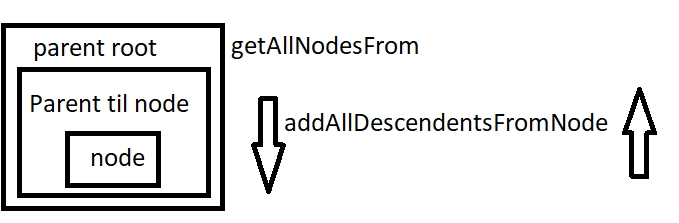
\includegraphics[scale = 0.7]{./PNG/imp/nodes.PNG} 
	\caption{Viser oprationen for hvordan den henter alle nodes}
	\label{fig:nodes}
\end{figure}
Createcase sender det map der består af de 3 maps til Domain, hvor dataene bliver valider efter om der er lavet en sagsobjektet med caseID eller der skal laves en ny sag. \\
I saveCase bliver det map splitte op i 3 map igen. Hvor der bliver lavet en validering af sags id. \\
\begin{figure}[hbt!]
\begin{lstlisting}
if (contentsMap.get("caseID").equalsIgnoreCase("-1")) {
	contentsMap.remove("caseID");
	caze = dataHandler.createCase();
	caze.setCaseContent(contentsMap);
	caze.setCaseStatus("Igang");
	caze.setRegardingCitizen(regardingCitizen);
	caze.setRequestingCitizens(requestingCitizenList);
	caze.setDepartmentID(departmentID);
} else {
	// TODO: If there is a case already you just need to set content (In regards to write it to the database)
	caze = null;
	System.out.println("TEST");
	return false;
}
\end{lstlisting}
\end{figure}

Denne del af metoden tjekker om der skal lave en ny sagsobjektet eller om dataene høre til en eksistere sagsobjektet. \\
Når det er gjort, vil sagsobjektet blive sendt til writeCase i datahandlern.\\
writeCase validere sags id og vis det er -1 vil en ny sag blive oprette i databasen med en timestame. \\
Dataene bliver tilførte til databasen gennem preparedstatemends.\\
Writecase sende en true tilbage gennem system til UI.\\
\textbf{Evaluering }\\
NodeFinder kan implementeres i alle fxml og samle den specifik data, hvis node id passer med det tablen i databasen. Dette gør at det bliver nemmer for fremtidige programøre at implementere fxml dokumenter i systemet og samle den data der bliver sat ind.\\
SaveCase 	\\
Opretter en ny borger uanset om borgen eksister. Den går ikke ned og tjekker om der er en borger med det givende cpr nr. den tjekker kun for sags id, hvilke gør at muligt at oprette flere sager på den enkelte borger. \\
\subsubsection{Search case}
\textbf{Problem} \\ 
Hvordan kan en Aktør finde en sag i databasen\\
\textbf{Eksempel}
\begin{figure}[hbt!]
\begin{lstlisting}
public Map<String, Map<String, String>> search(String key, String value) {
	value += "%" + String.valueOf(departmentID);
	IDataHandler searchHandler = new DataHandler();
    List<SearchCase> searchCases = searchHandler.search(key, value);

    int length = searchCases.size();

    Map searchResultList = new HashMap();
    for (int i = 0; i < length; i++) {
		Map searchResultMap = new HashMap();
        searchResultMap.put("citizenName", searchCases.get(i).getCitizenName());
        searchResultMap.put("currentCaseDate", searchCases.get(i).getCurrentCaseDate());
        searchResultMap.put("createdCaseDate", searchCases.get(i).getCreatedCaseDate());
        searchResultMap.put("caseReason", searchCases.get(i).getReason());
        searchResultMap.put("caseEmployeeName", searchCases.get(i).getEmployeeName());
        searchResultMap.put("caseStatus", searchCases.get(i).getCaseStatus());
        searchResultList.put(searchCases.get(i).getCaseID(), searchResultMap);
    }
    return searchResultList;
}
\end{lstlisting}
\end{figure}
\textbf{Løsning} \\
For at løst problemet er der blevet lavet search. Der er en metode der sender et efterspøgelse ned til Datahandler hvor den får en liste af objekter searchCases tilbage igen. \\
\begin{figure}[hbt!]
\begin{lstlisting}
public Map<String, Map<String, String>> search(String key, String value) {
	value += "%" + String.valueOf(departmentID);
}
\end{lstlisting}
\end{figure}
Her bliver der lavet en adskillendes mellem det forskellige afdelinger ved brugen af departmentID, hvilket er med til at lave en dataafgrænsning, der gøre at en afdeling kun kan se sager der tilhøre den afdeling.\\
Herefter lave der er objekt af datahandleren der skal bruge den en nøgle og den value der lave ud fra Department id.\\
Datahandleren har også en metode der hedder search. Hvor den laver en perparedStatement ved brugen af den key der kommer fra Department.  Og ud fra den værdi der bliver givet laver den setStrings hvor den switcher værdien med  ?  i Queryen.\\
Et Resultset bliver givet tilbage fra databasen og lagt ind i et nyt objekt searchCase.\\
Dette Objekt splitter Department til en liste af de resultater der kommer fra databasen.\\
Den data bliver sendt op gennem UI og synliggjort for aktøren.\\
\textbf{Evaluering}\\
Det gode ved den metoder er at den laver et object af search case der samler den data der kommer fra databasen. Hvilket giver beder mulig hed for at hente er specifikke data fra objektet. \\
